\chapter{Surface current and power loss in a conductor}\label{lec:lec28}
In our previous chapter, we talked about Power Flow in an electromagnetic wave and pointing vectors for electromagnetic waves. The Poynting vector tells us the density of power flow and its direction tells us the direction of the power at any location in space.

In this chapter, we will talk about surface current and power loss in a conductor.

We have always wondered how much power is lost in a conducting surface when an electromagnetic wave is incident on the conducting surface, the origin of surface current and if we really have surface current in practice and many more.

Surface Current is essentially a phenomenon which lies on the surface of the medium. This is a phenomenon which is for ideal conducting surfaces.

We will begin this chapter with the volume current density inside a conductor. We know the concept of skin depth in a good conductor, from there we will find out the current which is the surface current and see that, in practical systems the concept of surface current is very useful in finding out how much losses takes place in a conducting surface. First, we will discuss surface current and then go to power loss in a conducting surface.

We established that $\hat{n}$x$\hat{H}$ gives the direction of the surface current. $\hat{n}$x$\hat{H}$ gives us the direction which goes into the paper as shown in the figure~\ref{fig:direction_of_surface_current}
\begin{figure}[h]
\centering
\textsc{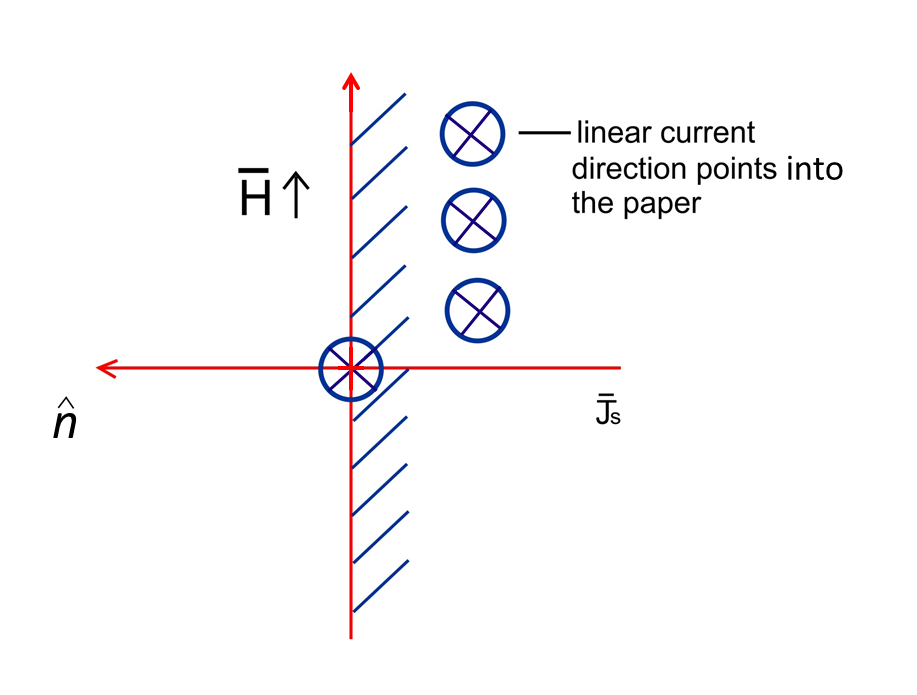
\includegraphics[width=1\linewidth]{\pathtopartone/graphics/surface_current_direction}}
\caption{Direction of the surface current}
\label{fig:direction_of_surface_current}
\end{figure}

This gives the linear surface density $\bar{J}$s we talked about when we dealt with boundary conditions. Now, if the surface current is flowing here, what is the driving mechanism for this surface current?

It is already established that this surface current phenomenon is associated with infinite conductivity. So if we take an ideal conductor, then maybe at some point if time, instantaneously, some electric fields existed in the medium and since it was a very short-lived phenomenon we had electric and magnetic fields together.

For the momentary existence of the electric field, it would put the charges into motion, which would constitute this current and since the conductivity is infinite, even if the electric field doesn't exist anymore when the charges are put in motion, the charges will keep moving for infinite time which constitutes a current. So when the conductivity is infinite, one may visualize that at some instant of time, some electric field induced motion to these charges. The charges were set in motion and they kept moving which is essentially the surface current and this is balanced by the magnetic field and $\hat{n}$x$\hat{H}$ essentially gave us that current density $\bar{J}$.

So basically, there are two situations now; (i) When we have a tangential component of electric field on the conducting surface which is zero but there are no surface currents and (ii) when the tangential component of electric field is zero but there is surface current. So in both situations, we have the tangential component of an electric field to be zero for ideal conductors but in one case, we have surface current and in the other case, we may not have surface current. If we have a surface current, then it must be balanced by the magnetic field. So if we have a magnetic field tangential to the conducting boundary, then we will have surface current otherwise we will not have surface current. This is a hypothetical situation of when surface current is truly flowing on the surface. Now, we may be curious to see what happens if we take a good conductor, whether we can still make use of this concept called surface current or not. It is very clear that if we have a conductivity which is not infinite, then because of the electric field, there will always be a finite conduction current density inside the material of the conductor. Also, the skin depth will be of finite width, which implies that this phenomenon is no more a true surface phenomenon (which requires zero thickness for skin depth). From the diagram of the conductor shown below, let \textbf{z} \textgreater 0 represent the conductor.
\begin{figure}[h]
\centering
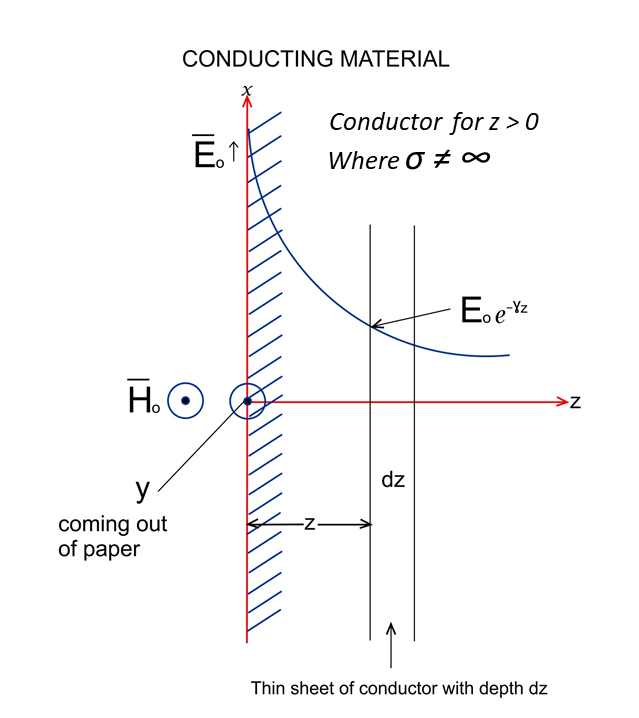
\includegraphics[width=0.9\linewidth]{\pathtopartone/graphics/thin_sheet_conductor}
\caption{Exponential decay of electric field inside a conductor}
\label{fig:exponential_decay_of_E_in_conductor}
\end{figure}	

If we have an electric field in this conductor for a finite $\sigma$ not equal to $\infty$, then the tangential component of \textbf{E} on this surface is not zero (very small but not zero as for an ideal conductor with $\infty$ conductivity). Let \textbf{E} be in \textbf{x} direction and \textbf{H} in \textbf{y} direction. The electric field \textbf{E} dies down exponentially as we go into the conductor as shown in fig\ref{fig:exponential_decay_of_E_in_conductor}. \textbf{E} dies down at $e^{-\gamma z}$. Once we know the electric field value at the surface of the conductor, we have
\begin{align}
\gamma=\sqrt{\textit{j}\omega\mu\sigma}
\end{align}
for a good conductor, $\sigma$ is very large. $\gamma$=$\alpha$+$j\beta$ to get
\begin{align}
\gamma=\sqrt{\frac{\omega\mu\sigma}{2}}+\textit{j}\sqrt{\frac{\omega\mu\sigma}{2}}=\alpha+\textit{j}\beta
\end{align}

Since the current flow is in the direction of the electric field $\hat{x}$, we have a conduction current density $\bar{J}$=$\sigma\bar{E}_0$ which varies exponentially as we go deeper inside the conductor. We can take a thin sheet with a depth of \textbf{dz}. The conduction current is thus, $\bar{J}$=$\sigma\bar{E}_0$e$^{-\gamma z}$. So if we know the current flowing in the sheet per unit area in the xy plane, we can find out the total current flowing through the surface of the xy plane in the x direction. So if we take the conduction current density and integrate it over the depth, we get the total current flowing through the surface xy. If we take that surface as a unit surface, then the current that is flowing is with respect to that unit area. So for the dz region, the conduction current density;

$\bar{J}$(z) = $\sigma$$\bar{E}$ = $\sigma\bar{E}_0e^{-\gamma z} \hat{x}$ = $\sigma\bar{E}_0$e$^{-\alpha z}$e$^{-j\beta z}$.\\
Unit depth in the y direction and width dz represents the area that $\bar{J}$ flows through. For this Area$=1\times dz=dz$. Since the current flows in $\hat{x}$ direction, the area normal to this flow is in the yz plane and thus we take a unit y depth. So, current in a sheet of unit depth in the y direction along the whole z plane is determined by integrating over the entire z.

\begin{dmath}
\textbf{I}(z)=\bar{J}(z)\times Area 
=\bar{J}(z)dz 
=\sigma\bar{E}_0e^{-\gamma z}dz \hat{x}
\end{dmath}
This equation is the current per unit length in the y direction. The total current flowing on the surface is the surface current. Note that there is no true surface current, the current flow into the depth of z but dies down very fast. Hence the little current flow is limited to small dz on the surface of the conductor with large conductivity, we know that the skin depth is very small, so the current flow is confined to the surface, but not truly confined to the surface to a skin depth from the surface;
Surface current,
\begin{dmath}
\bar{J}_s=\int\limits_0^\infty\sigma\bar{E}_0 e^{-\gamma z}dz\hat{x}
=\frac{\sigma\bar{E}_0}{-\gamma}[e^{-\gamma z}]_0^\infty \hat{x}=\frac{\sigma}{\gamma}\bar{E}_0\hat{x}
\end{dmath}
Though we call $\bar{J}$s surface current density, it is clear that it is not truly a surface phenomenon but it has all the properties which a surface current has. And one of such properties is that the surface current should be related to a magnetic field, that is, the tangential component of the magnetic field to the surface and it should satisfy the relationship of $\hat{n}\times\hat{H}=\bar{J}_s$. 

So if 
$\bar{J}=\dfrac{\sigma}{\gamma}\bar{E}_0\hat{x}$ must serve as surface current density, it must be related to the magnetic field and satisfy the relationship $\hat{n}$x$\hat{H}$=$\bar{J}$s.

Since we have an electric field which is $\bar{E}$$_0$ on the surface and magnetic field $\bar{H}$$_0$, with the wave travelling inwards in the z-direction, being a transverse electromagnetic wave as the medium is unbound, then $\dfrac{\bar{E}_0}{\bar{H}_0}$ must satisfy the relationship of being of equal to the intrinsic impedance of the medium.
For a good conductor, intrinsic impedance
\begin{align}
\eta_{c}=\sqrt{\dfrac{j\omega\mu}{\sigma}} 
\end{align} 
And the electric and magnetic field are related by $H_0=\dfrac{E_0}{\eta_{c}}$
but $\gamma =\sqrt{j\omega\mu\sigma}$\ so,
\begin{align}
\eta_{c}=\sqrt{\dfrac{j\omega\mu}{\sigma}}\equiv\sqrt{\dfrac{j\omega\mu\sigma}{\sigma^{2}}}=\dfrac{\gamma}{\sigma}
\end{align}
Hence,
\begin{align}
\bar{H_{0}}=\dfrac{\bar{E_0}}{\eta_{c}}=\dfrac{\sigma \bar{E_0}}{\gamma}
\end{align}
But this quantity is the same as what we got for the surface current density $\bar{J_{s}}$ earlier; \\
$\bar{J}_s=\dfrac{\sigma}{\gamma}E_0\hat{x}$ \\
Thus,
\begin{align}
\lvert H_0\rvert=\dfrac{\sigma}{\gamma}\lvert E_0\rvert=\lvert \bar{J}s\rvert.
\end{align}

So one relationship we wanted was that if $\bar{J}_s$ is surface current density the way we have visualized it, then it must be related to the magnetic field which we have proven as $\lvert H_0\rvert=\lvert\bar{J}_s\rvert$. The second requirement is that $\hat{n}\times\hat{H}=\bar{J}_s$ i.e $\hat{n}\times\hat{H}$  must give surface current direction. $\hat{J_{s}}$ was in direction of \textbf{E} that is $\hat{x}$. So we have a surface current density $\hat{J_{s}}$ direction that is  $\hat{x}$ oriented and a magnetic field \textbf{H} that is $\hat{y}$ oriented. The unit normal to the conducting surface is $\hat{n}$ = $-\hat{z}$. Now;
\begin{equation*}
\hat{n} \cross \hat{H} = -\hat{z} \cross H_{0}\hat{y} = H_{0}(-\hat{z} \cross \hat{y})
\end{equation*}
but $-\hat{z} \cross \hat{y}$ gives $\hat{x}$ direction which is the direction of $\bar{J_{s}}$
thus, $\bar{J}_s = \dfrac{\sigma}{\gamma}E_0\hat{x}$ has all the characteristics of a surface current density. The magnitude of the magnetic field should be equal to that of the surface current density. It becomes obvious that, though $\bar{J}$s=$\dfrac{\sigma}{\gamma}$$E_0$$\hat{x}$ is not a true surface current, we still use it as a surface current nonetheless.

Also when conductivity is very large, this current is effectively confined to a very thin layer called skin depth. As we have seen earlier, if we go to frequencies like 300MHz, skin depth lies in a few micron range. So essentially this is a current flowing through a very thin sheet on the surface of the conductor. Also, it has the characteristics of a true surface current that is, it is related to the magnetic field and $\hat{n}$ x $\bar{H}$ gives its direction. So this quantity can be used as the surface current in a good conductor. Although in the true sense, there is no surface current for a good conductor, in practice, we make use of the quantity $\bar{J_{s}}$ as surface current in our analysis.

Once we get surface current, we define a quantity called \textbf{SURFACE IMPEDANCE} which is a boundary parameter for this boundary. This is useful whenever we do the power calculation on a conducting surface.

\begin{align}
\text{Surface impedance, }Z_{s}=\dfrac{E_{tangetial}}{\bar{J}s}
\end{align}
\begin{align}
\bar{J}s=\dfrac{\sigma}{\gamma}E_0\hat{x}
\end{align}
$\bar{J_{s}}$ has a unit of $\dfrac{A}{m}$, that is, linear surface current density.
To determine the unit of $Z_{s}$, we have;
\begin{align}
Z_{s}=\dfrac{V/m}{A/m}=\dfrac{V}{A}=\Omega
\end{align}
So as expected, the quantity Z$_{s}$ is some form of impedance. If we know the tangential component of the electric field, then the surface current can be obtained from what is called the surface impedance or vice versa.
\begin{align}
Z_{s}=\dfrac{E_0}{\dfrac{\sigma}{\gamma} E_0}=\dfrac{\gamma}{\sigma}=\dfrac{\sqrt{j\omega\mu\sigma}}{\sigma}=\sqrt{\dfrac{j\omega\mu}{\sigma}}=\eta_{c}
\end{align}
So for a good conductor, the intrinsic impedance of the medium is the same as the surface impedance. Later we will see that the surface impedance concept is used to calculate the power loss. Now if we know the tangential component of the electric field and know the conductivity, we can calculate the intrinsic impedance of the medium which is the same as the surface impedance.
Once we have the surface current density $\bar{J}$s, then we ask how much is the power loss due to this surface current density flowing in this conductor. Considering the surface of the unit area, how much is the power loss in this unit area of the conducting surface? Since the current is flowing into the depth of the conductor, the power loss is not only taking place on the surface, it takes place all along the depth of the conductor. So to determine the total loss, we take the total depth of the conductor, and a unit area of thickness dz as shown below.

\begin{figure}
\centering
\textsc{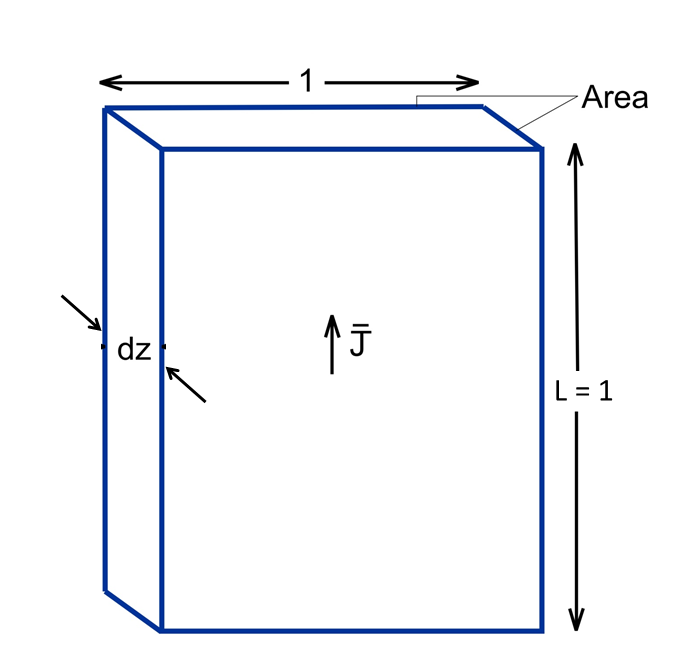
\includegraphics[scale=0.35]{\pathtopartone/graphics/slab_parallel_to_conducting_surface}}
\caption{A thin slab layer of thickness dz parallel to the surface of the conductor }
\end{figure}
So if we take a thin slab parallel to the surface of the conductor, since we have a finite conduction current, we ask how much the power loss is in this thin slab. If we integrate over all depth z, we get the power loss per unit area on the surface of the conductor.

All we need to do is to determine the surface current flowing and the resistance of the thin slab.
\begin{align*}
\bar{J}_s(1\times\mathbf{dz})\text{ is the current flowing in the direction of } \bar{J_{s}}
\end{align*}

\begin{center}
The length L is unity,
$\sigma$=conductivity,
$\dfrac{1}{\sigma}$= resistivity
\begin{dmath*}
\text{Resistance} = \dfrac{\text{Resistivity} \times \text{Length}}{\text{Area}}=\dfrac{1}{\sigma}\times\dfrac{1}{dz}=\dfrac{1}{\sigma dz}
\end{dmath*}
current flowing in the area $=Jdz, R=\dfrac{1}{\sigma dz}, I=Jdz, d\omega$ = ohmic loss in slab \\
$d\omega=\dfrac{1}{2}={\lvert I\rvert}^{2}R$, 
I and R can be complex hence $\dfrac{1}{2}{\lvert I\rvert}^{2}R$.
\begin{align*}
I=\bar{J}dz \text{ and } \bar{J} = \sigma E_{0} e^{-\gamma z}
\end{align*}
\begin{align*}
I=\sigma\bar{E}_{0}e^{-\gamma z}dz
\end{align*}
\begin{align*}
d\omega=\dfrac{1}{2}\lvert\sigma\bar{E}_{0}e^{-\alpha z}e^{-j\beta z}\rvert^{2}\times\dfrac{1}{\sigma dz}
\end{align*}
\begin{align*}
d\omega=\dfrac{1}{2}\sigma\lvert\bar{E}_{0}\rvert^{2}e^{-2\alpha z}dz
\end{align*}
\end{center}
The total power loss in the whole depth under the unit area of the surface becomes,
\begin{align}
\omega=\int_{0}^{\infty}\dfrac{1}{2}\sigma\lvert E_{0}\rvert^{2}e^{-2\alpha z}dz=\dfrac{1}{2}\sigma\bar{E}_{0}^{2}[\dfrac{e^{-2\alpha z}}{-2\alpha}]_{0}^{\infty}
\end{align}
\begin{align}
\omega=\dfrac{1}{2}\dfrac{\sigma}{2\alpha}\lvert E_{0}\rvert^{2}
\end{align}
but
\begin{align}
\gamma=\sqrt{j\omega\mu\sigma}=\alpha+j\beta=\sqrt{\dfrac{\omega\mu\sigma}{2}}+j\sqrt{\dfrac{\omega\mu\sigma}{2}}
\end{align}
So $\alpha = \sqrt{\frac{\omega\mu\sigma}{2}}$
\begin{align}
w = 	\dfrac{1}{2}\times\dfrac{\sigma}{2\sqrt{\dfrac{\omega\mu\sigma}{2}}}\times\lvert E_{0}\rvert^{2}
\end{align}
recall, $\bar{J_{s}} = \frac{\sigma}{\gamma}E_{0}\hat{x}$\\
so, $\lvert E_{0}\rvert^{2} = \frac{\lvert \gamma\rvert ^{2}}{\lvert \sigma\rvert^{2}}\lvert \bar{J_{s}}\rvert^{2}$
\begin{align}
w = \frac{1}{2}\times\dfrac{\sigma}{2\sqrt{\dfrac{\omega\mu\sigma}{2}}}\times \frac{\lvert \gamma\rvert ^{2}}{\lvert \sigma\rvert^{2}}\lvert \bar{J_{s}}\rvert^{2} 
\end{align}
\begin{align*}
w = \frac{1}{2}\times\frac{1}{2}\sqrt{\frac{2}{\omega\mu\sigma}}\times\omega\mu\times\lvert \bar{J_{s}}\rvert^{2}
\end{align*}
\begin{align}
w = \frac{1}{2}\sqrt{\frac{\omega\mu}{2\sigma}}\lvert\bar{J_{s}}\rvert^{2}
\end{align}

\begin{align}
Z_{s}=\sqrt{\dfrac{j\omega\mu}{\sigma}}=\sqrt{\dfrac{\omega\mu}{2\sigma}}+j\sqrt{\dfrac{\omega\mu}{2\sigma}}
\end{align}
Hence we say that the surface impedance has a resistive part called the surface resistance and a reactive part called the surface reactance.
\begin{align}
Z_{s}=R_{s}+jX_{s}\\	
\omega=\dfrac{1}{2}\times \lvert\bar{J}s\rvert^{2}\times \sqrt{\dfrac{\omega\mu}{2\sigma}}=\dfrac{1}{2}\lvert\bar{J}s\rvert^{2}R_{s}
\end{align}

Thus, the power loss per unit area of conducting surface can be obtained if we know the surface current density and the surface resistance.

Later on, we would see that if we go to structures like waveguides, then the conductor loss is calculated from the surface current density because the conductor surface current density can be obtained from magnetic fields. So if we know the tangential component of the magnetic field on the surface of the conductor, we can find out using $\hat{n}\times\bar{H}$, the linear surface current density with $\bar{J}_s$ known and $Z_{s}$(surface impedance) known, from there we can find out the power loss per unit area of the conductor.

Essentially we have calculated the power loss by using the circuit concept that is, we found out the current and the resistance in the slab, then we found out the $I^{2}R$ loss, and from there we obtained the power loss on the surface of the conductor. We can also determine the power loss by using the wave approach. Once we have an electric and magnetic field, there is essentially a wave phenomenon going in the z-direction. So the power going with the wave into the conductor is essentially the power which is lost into the ohmic loss conductor. This power is finite and is decreasing as the wave travels with time as no power is coming back. So whatever the power flow inside the conductor is, is a measure of the power that was lost inside the conductor. So instead of doing the calculation of the power loss from an electrical point of view, by finding out the current and resistance, we can use the wave concept and find out what the power loss is inside the conductor with the interface and \textbf{E} and \textbf{H} being in the directions shown in the figure below. Since we are asking for power flow per unit area of the surface, we find the Poynting vector at the surface of the conductor. That is the power which is essentially going into the conductor and which is lost as Ohmic losses in the conductor.

\begin{figure}
\centering
\textsc{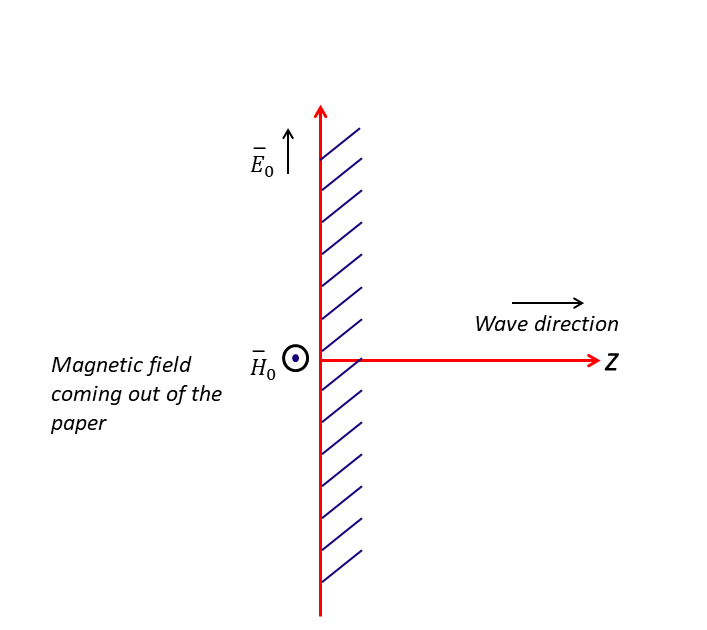
\includegraphics[width=0.9\linewidth]{\pathtopartone/graphics/power_flow}}
\caption{Determination of the power loss using wave concept}
\end{figure}

Poynting vector,
\begin{align}
\bar{P}=\bar{E}\times \bar{H}=\dfrac{1}{2}\mathfrak{Re}(E_{0}H_{0}^{\ast}\hat{z})
\end{align} 
We substitute $\bar{H}$$_{0}$=$\dfrac{E_{0}}{\eta_{c}}$ for this medium
\begin{align}
\bar{P}=\dfrac{\lvert\bar{E}_{0}\rvert^{2}}{2\eta_{c}^{\ast}},\quad
\bar{P}=\dfrac{1}{2}\lvert\bar{E}_{0}\rvert^{2}\times \dfrac{1}{\eta_{c}^{\ast}}
\end{align}

Recall  $\eta_{c}=\sqrt{\dfrac{j\omega\mu}{\sigma}}$
So that,\\
$\eta_{c}=\sqrt{\dfrac{\omega\mu}{\sigma}}(\dfrac{1}{\sqrt{2}}+j\dfrac{1}{\sqrt{2}})$\\
$\eta_{c}^{\ast}=\sqrt{\dfrac{\omega\mu}{\sigma}}(\dfrac{1}{\sqrt{2}}-j\dfrac{1}{\sqrt{2}})$\\

$\eta_{c}=\sqrt{\dfrac{\omega\mu}{\sigma}}(\dfrac{1}{\sqrt{2}}+j\dfrac{1}{\sqrt{2}})$\\
$\eta_{c}^{\ast}=\sqrt{\dfrac{\omega\mu}{\sigma}}(\dfrac{1}{\sqrt{2}}-j\dfrac{1}{\sqrt{2}})$\\
\begin{align}
\bar{P}=\dfrac{1}{2}\lvert\bar{E}_{0}\rvert^{2}{\frac{1}{\sqrt{\dfrac{\omega\mu}{\sigma}}(\dfrac{1}{\sqrt{2}}-j\dfrac{1}{\sqrt{2}})}} 
\end{align}
$=\dfrac{1}{2}\lvert\bar{E}_{0}\rvert^{2}\times \dfrac{\sqrt{\dfrac{\omega\mu}{\sigma}}(\dfrac{1}{\sqrt{2}}+j\dfrac{1}{\sqrt{2}})}{\sqrt{\dfrac{\omega\mu}{\sigma}}(\dfrac{1}{\sqrt{2}}-j\dfrac{1}{\sqrt{2}})\times \sqrt{\dfrac{\omega\mu}{\sigma}}(\dfrac{1}{\sqrt{2}}+j\dfrac{1}{\sqrt{2}})}$\\\\
$\bar{P}=\dfrac{1}{2}\lvert\bar{E}_{0}\rvert^{2}\mathfrak{Re}\left\lbrace\dfrac{\sqrt{\dfrac{\omega\mu}{\sigma}}\left(\dfrac{1}{\sqrt{2}}+j\dfrac{1}{\sqrt{2}}\right)}{\dfrac{\omega\mu}{\sigma}\left(\dfrac{1}{2}+\dfrac{1}{2}\right)}\right\rbrace\\\\
\bar{P}=\dfrac{1}{2}\lvert\bar{E}_{0}\rvert^{2}\mathfrak{Re}\left\lbrace\dfrac{\sigma}{\omega\mu}\left(\sqrt{\dfrac{\omega\mu}{\sigma}}\left(\dfrac{1}{\sqrt{2}}+j\dfrac{1}{\sqrt{2}}\right)\right)\right\rbrace$\\\\
$\bar{P}=\dfrac{1}{2}\lvert\bar{E}_{0}\rvert^{2}\times \sqrt{\dfrac{\sigma}{\omega\mu}}\times \dfrac{1}{\sqrt{2}}$\\\\
\begin{equation}
\bar{P}=\dfrac{1}{2}\lvert\bar{E}_{0}\rvert^{2}\times \sqrt{\dfrac{\sigma}{2\omega\mu}}
\end{equation}

This expression is the same as we got for power loss using the surface impedance of the conducting medium. So we can calculate the power loss either by using the circuit concept or the wave concept. Using the circuit concept, we find $\bar{J}$$_{s}$ and find out the ohmic loss or $I^{2}R$ loss using the wave concept, we find out what the power going inside the surface of the conductor is and that power should essentially get lost inside the conductor. Since the field at $z=\infty$ goes to zero there is no power flow at $z=\infty$, so whatever power went into the conductor must have been lost in the heating of the conductor. So either the electrical circuit concept or the wave concept can be used to find out the power loss per unit area on the surface of the conductor.

The power that is being lost inside the conductor is proportional to the conductivity from $P=\dfrac{1}{2}\lvert E_{0}\rvert^{2}\sqrt{\dfrac{\sigma}{2\omega\mu}}$.
We are dealing with electromagnetic waves here, SO The higher the conductivity of the medium it propagates in, the more the power loss of this wave so that in a pure dielectric with $\sigma$=0, it will have no power loss in that medium. So, large $\sigma$ means a large part of the electromagnetic wave energy is taken by the medium (or lost to the medium). With high frequency, it losses less of its energy to the medium through which it propagates. So for an ideal conductor with $\sigma\longrightarrow\infty$, the EM wave losses all of its power to this conductor but with skin depth of nearly zero, all of this energy lost flow as pure surface current on this conductor without any Ohmic losses and the entire energy is reflected from the boundary.
\footnote{
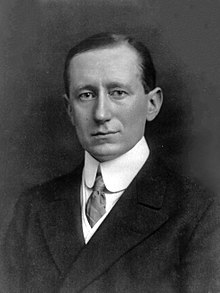
\includegraphics[height=20mm]{\pathtopartone/graphics/footnotegm.jpg}

Guglielmo Marconi, 1st Marquis of Marconi (25 April 1874 - 20 July 1937) was an Italian inventor and electrical engineer known for his pioneering work on long-distance radio transmission and for his development of Marconi's law and a radio telegraph system. He is usually credited as the inventor of the radio
}

For an ideal conductor, there is no power going inside the conductor similarly when the frequency becomes large, there is no power going inside the conductor. What this means is that, for high conductivity or high frequency, there is a resistance to the penetration of the conductor, hence, the power does not go inside the conductor.

This situation is similar to a lossy transmission line but however, in a lossy transmission line, the power gets lost in the heating of the line. In this case, the power is dying down rapidly but the power is not lost in the Ohmic loss because the power is not able to penetrate the layer. So for conductivity = $\infty$, no power penetrates the conductor so it gets reflected.

In conclusion, when the conductivity is infinite, the wave does not penetrate the medium, there is no power loss and the entire energy is reflected from the boundary.
